\documentclass[../main.tex]{subfiles}

% ======================== Preamble ================================================%

% ======================== Document: Appendix B: Patent parties models ======================== %

\begin{document}
\section{Appendix: Patent parties models}
\label{sec:appendixb}

\begin{table}[htbp!]
    \centering
\begin{threeparttable}
    \caption{Difference-in-differences specifications for quarterly patent parties}
    \label{tab:dd_twfe_patents_parties}
    
\begin{tabular}[t]{lcccc}
\toprule
  & (1) & (2) & (3) & (4)\\
\midrule
DD & \num{0.082} & \num{0.149} & \num{0.007} & \num{0.012}\\
\textbf{} & \textbf{(\num{0.101})} & \textbf{(\num{0.117})} & \textbf{(\num{0.079})} & \textbf{(\num{0.096})}\\
\midrule
Party type & Total & Inventors & Applicants & Owners\\
$N$ & \num{656} & \num{656} & \num{656} & \num{656}\\
Adj. $R^2$ & \num{0.974} & \num{0.969} & \num{0.969} & \num{0.971}\\
Adj. within $R^2$ & \num{0.136} & \num{0.130} & \num{0.094} & \num{0.148}\\
RMSE & \num{0.210} & \num{0.229} & \num{0.220} & \num{0.228}\\
\bottomrule
\end{tabular}
}
    \begin{tablenotes}
        \small
        \item \textit{Notes}: All specifications include controls in Specification (3) of Table \ref{tab:dd_twfe_patents}, not shown for brevity and fixed effects for provinces and quarters. Clustered standard errors at the province and quarter level shown in parentheses. ***$p<0.01$, **$p<0.05$, *$p<0.1$.
    \end{tablenotes}
\end{threeparttable}
\end{table}

\begin{figure}[htbp!]
    \centering
    \caption{Event study plot for quarterly parties in patent parties}
    \label{fig:event_study_patent_parties}
    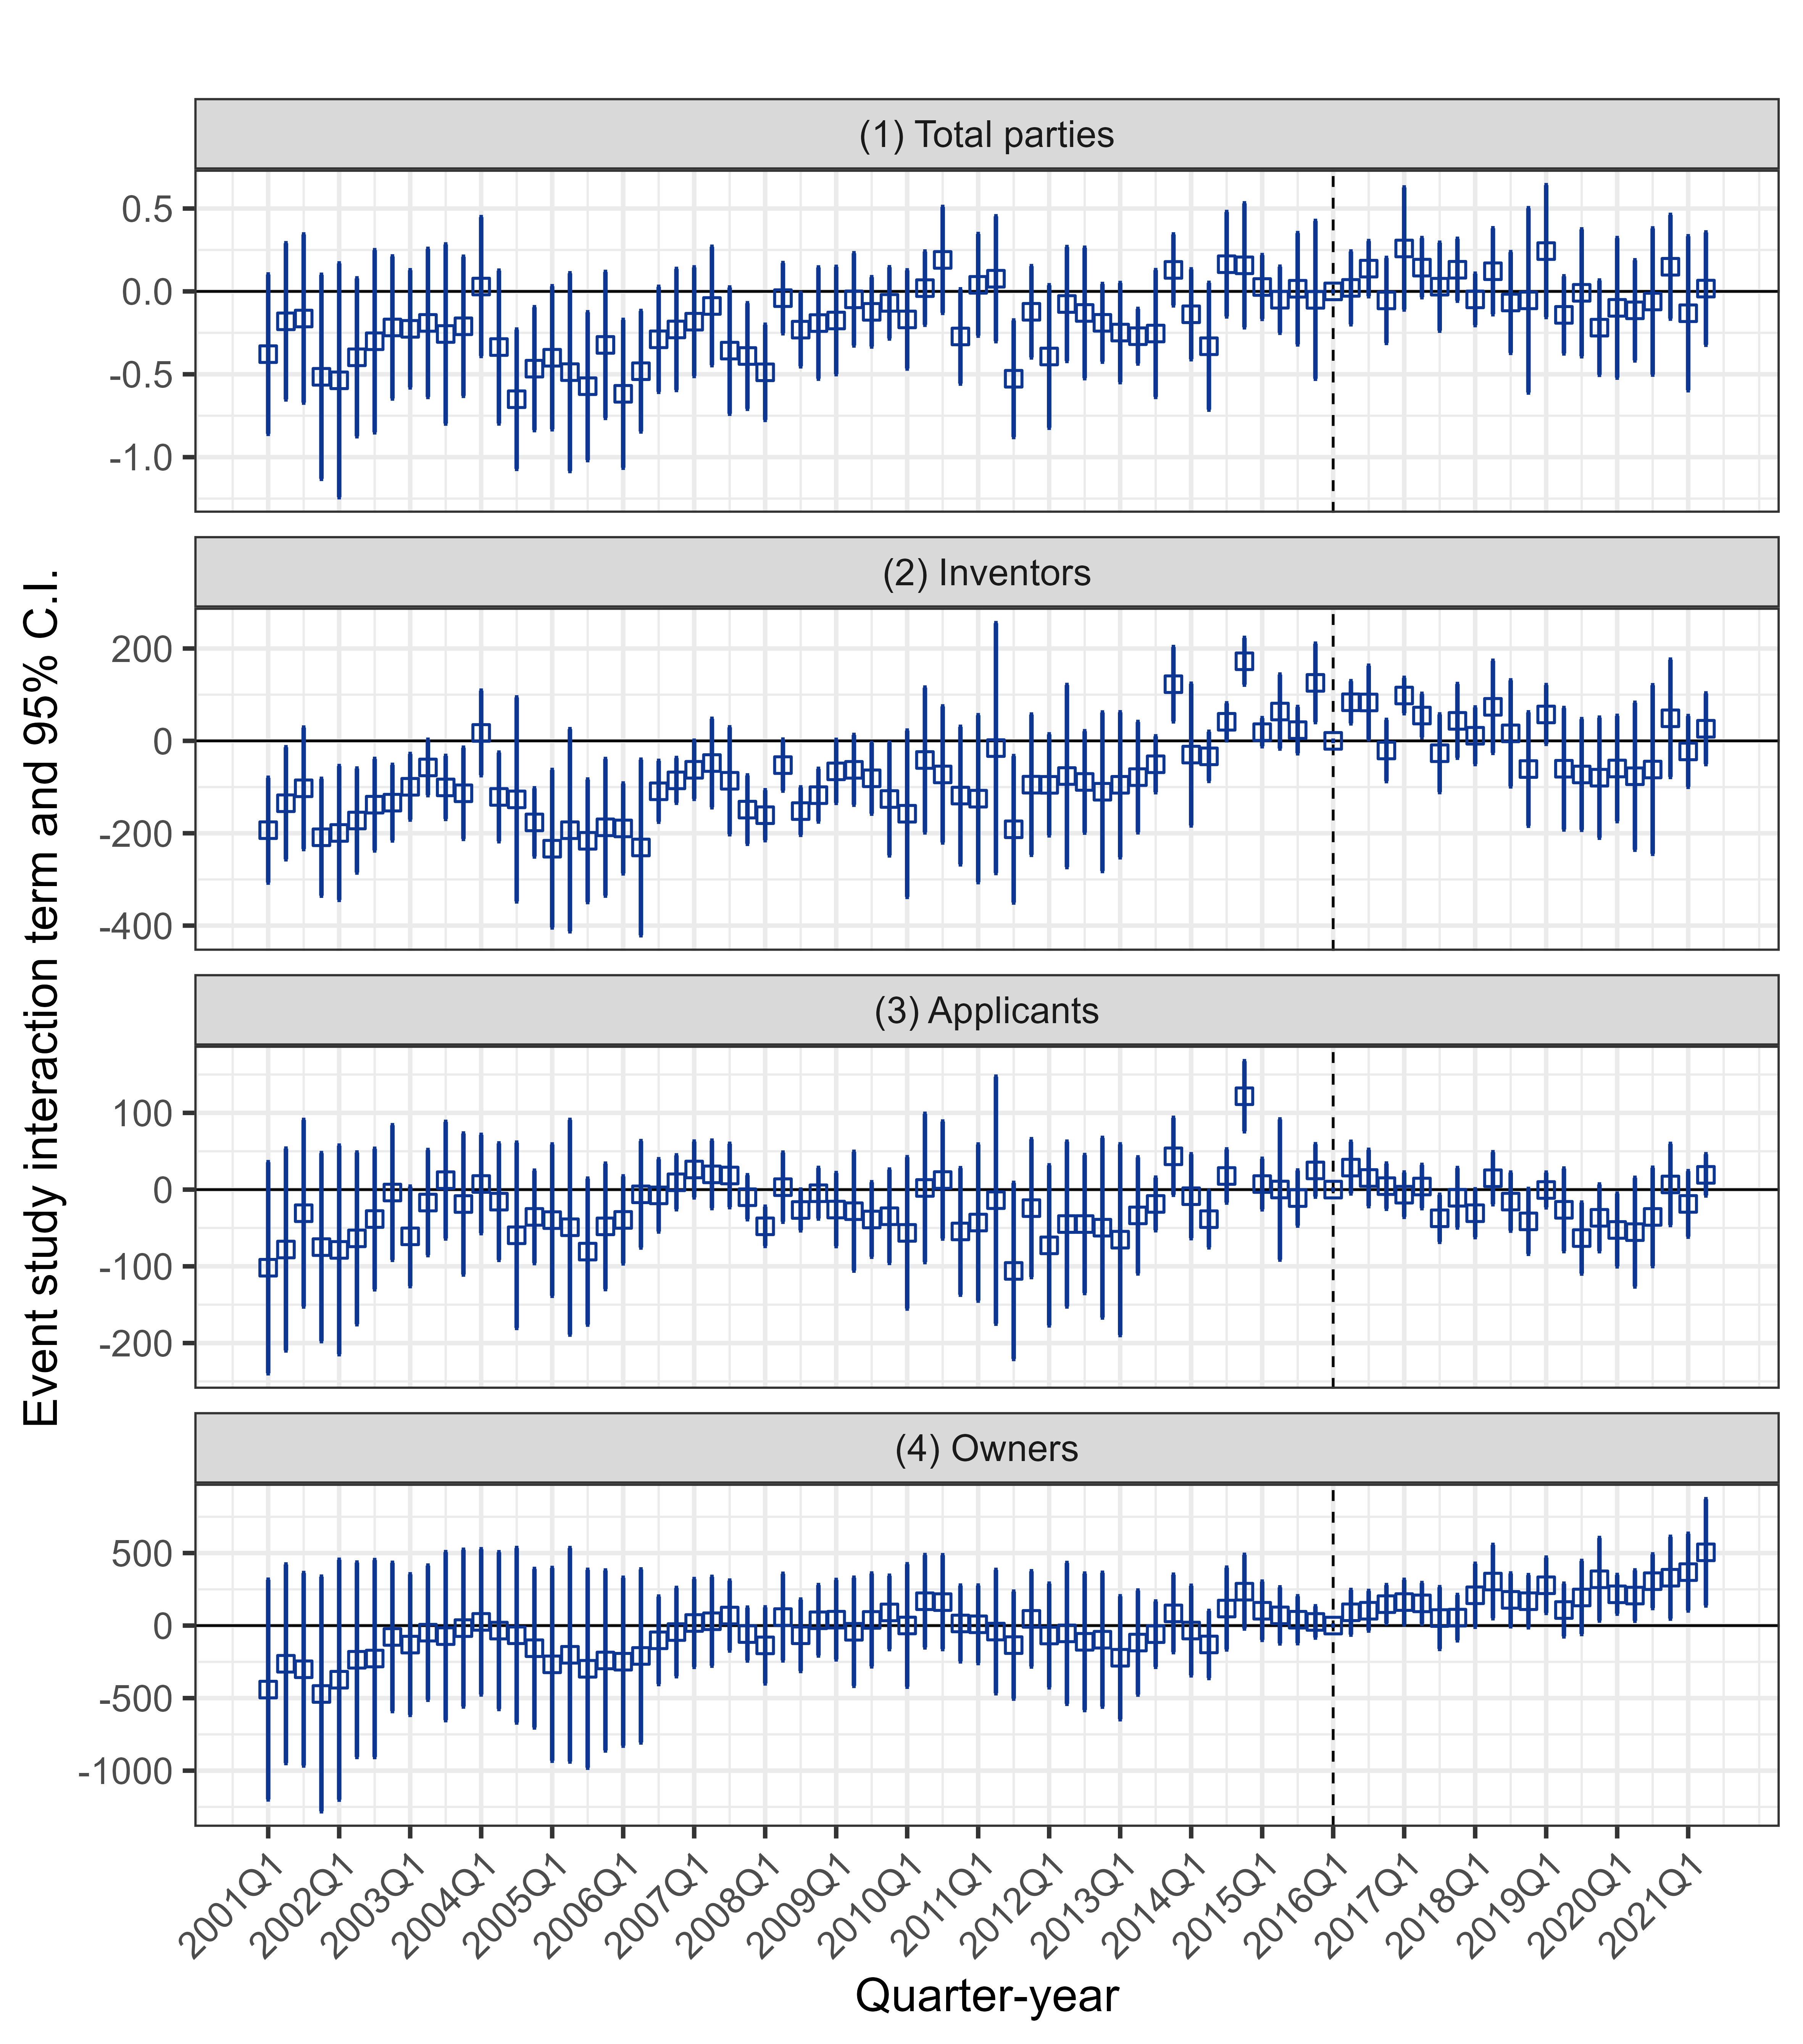
\includegraphics{\subfix{../../figures/event-studies/quarterly/parties_faceted.png}}
    \begin{minipage}{0.9\textwidth}
        \footnotesize
        \textit{Notes}: The figure shows the estimated coefficients of the interaction term between period and treatment binary variables in Equation \ref{eq:event_study} for each quarter. The points represent the point estimate, while the error bars represent the 95\% confidence cluster-robust interval. The vertical line represents the start of the AITC intervention in 2017Q1, with the reference level being the quarter before the intervention. Baseline, economic, and additional controls specifications include the controls seen in specifications (1) through (3) in Table \ref{tab:dd_twfe_patents}. 
    \end{minipage}
\end{figure}



\end{document}